\chapter{Sistema TRUE}
\label{cap:true}

% inciailmetne explicar q ambiente inteligentes sao viabilizados por middleware de comput ubi
% apresentar ups caracteristacas gerencias ambientes
% esse trabalho tem por objetivo desenvolver uma solcuao de ... para ambientes inteligentes gerecnaisdos pelo middleaew
% falar dos trbaalhos q desenvovlem solucoes semelhantes mas sao especificas para detemrinado ambiente
% primeira iniciativa trazer essa solucao para o middlewarel

% essa mono mais rpecisamente apresenta isso .... e acabouse desenvovlendo tres modulos, foram conduzidos tb testes bla bla bla


Um ambiente inteligente pode ser composto por uma grande variedade de dispositivos, que fornecem ao ambiente recursos. Para que estes se agreguem as tarefas do usuário, a inteligência presente deve coordená-los de acordo com as informações sobre o ambiente e sobre o usuário~\cite{fabriciobuzzeto}. Portanto, informações como posição do usuário e sua respectiva identidade são de grande valia para tornar possível a interação entre o usuário e os recursos presentes. Além disso, informações como estas ainda não são obtidas em ambientes inteligentes gerenciados pelo Middleware \textit{uOS}, apresentado na Seção~\ref{uos}. Atualmente, a maioria das soluções encontradas para fornecer esse tipo de informação foram projetadas para funcionar em ambientes rigidamente definidos. Com isso, não seria adequado tentar incorporar soluções como estas em um ambiente com diferentes dimensões, condições de iluminação, posição dos móveis, diferentes sensores pois este resultaria em um cenário diferente.

Esse trabalho propõe um sistema aberto de rastreamento, localização e identificação de pessoas em ambientes inteligentes gerenciados middleware \textit{uOS}. Tal sistema é chamado de TRUE, \textit{\textbf{T}racking and \textbf{R}ecognizing \textbf{U}sers in the \textbf{E}nvironment}. Ele consiste na primeira tentativa de se trazer informações de contexto contendo perfis e posições dos usuários para o middleware \textit{uOS}.


% Observando a realidade de um ambiente inteligente fica claro que as informações como posição das pessoas e suas respectivas identidades são de grande valia para que decisões possam ser tomadas. Atualmente, a maioria das soluções encontradas para fornecer esse tipo de informação foram projetadas para funcionar em ambientes rigidamente definidos. Com isso, não seria adequado tentar incorporar soluções como estas em um ambiente com diferentes dimensões, condições de iluminação, posição dos móveis, diferentes sensores pois este resultaria em um cenário diferente. Além disso, seria interessante que a solução fosse integrada com o middleware \textit{UbiquitOS} (Seção~\ref{uos}), disponibilizando, então, as informações obtidas dos usuários as diversas aplicações presentes no ambiente.

% Além disso, a solução deve ser integrada com o middleware \textit{UbiquitOS}, o qual gerência os serviços providos pelo ambiente inteligente.

% Esse trabalho propõe, então, um sistema aberto de rastreamento, localização e identificação de pessoas em um ambiente inteligente integrado com o middleware \textit{uOS}. Tal sistema é chamado de TRUE, \textit{\textbf{T}racking and \textbf{R}ecognizing \textbf{U}sers in the \textbf{E}nvironment}.

O Sistema TRUE é um sistema monomodal implementado em C++ que utiliza somente dados visuais, como imagens de cor e profundidade. As imagens de profundidade são utilizadas no rastreamento e localização dos usuários no ambiente, enquanto que as imagens de cor são utilizadas no reconhecimento facial e no cadastro dos usuários. Assim, o dispositivo de coleta de imagens presentes no ambiente deve ser capaz de fornecê-las a um taxa e qualidade adequadas. Para tanto, o sistema utiliza o sensor \textit{Kinect} da marca Microsoft descrito no Apêndice~\ref{sec:kinect}. O \textit{Kinect} é um dispositivo bastante acessível de custo aproximadamente \$150,00 e capaz de fornecer imagens de cor e de profundidade sincronizadas.

O Sistema TRUE é dividido em quatro módulos principais:

	\begin{itemize}
		\item \textbf{Módulo de Rastreamento}: responsável pelo rastreamento e localização dos usuários no ambiente.
		\item \textbf{Módulo de Reconhecimento}: responsável por identificar os usuários rastreados.
		\item \textbf{Módulo de Registro}: responsável pelo cadastro de novos usuários e treino do sistema.
		\item \textbf{Módulo de Integração}: responsável pela integração e comunicação do sistema com o Middleware \textit{uOS}.
	\end{itemize}

Basicamente, o Módulo de Rastreamento obtém o dados do sensor \textit{Kinect} que são utilizados nas tarefas de rastreamento e localização de cada usuário no ambiente. Quando necessário ele requisita ao Módulo de Reconhecimento a identificação de algum usuário repassando imagens do mesmo. Por sua vez, o Módulo de Reconhecimento acessa o banco de faces, contendo as faces das pessoas cadastradas no sistema, e identifica o usuário mais parecido retornando seu nome ao Módulo de Rastreamento. Este último, repassa as informações de cada usuário ao Middleware \textit{uOS} através do Módulo de Integração. Quando for necessário cadastrar um novo usuário no Sistema TRUE, o Middleware acessa o Módulo de Registro, também através do Módulo de Integração, que insere as imagens da nova pessoa na base de faces e retreina o sistema. A Figura~\ref{fig:relacao-modulos} ilustra essa interação entre os módulos do Sistema TRUE.

	\begin{figure}[htb]
			\begin{center}
				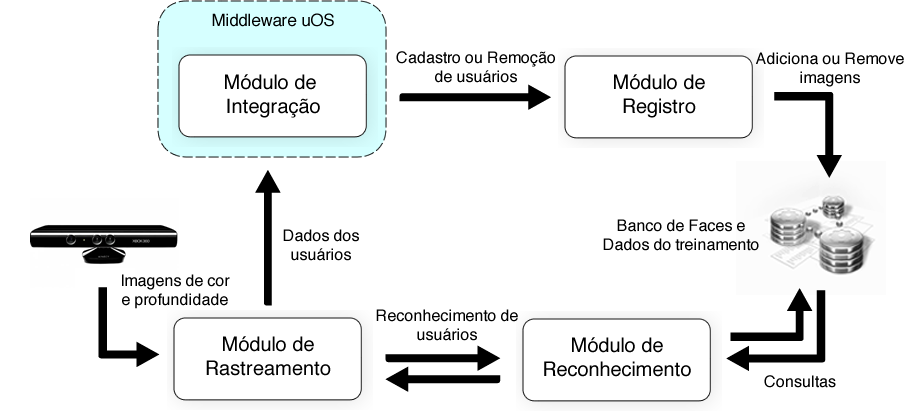
\includegraphics[scale=0.5]{figuras/4.ProblemaEProposta/modulo-integracao.png}
			\end{center}
			\caption{Interação entre o módulos do Sistema TRUE.}
			\label{fig:relacao-modulos}
		\end{figure}

A seguir serão apresentados em detalhes cada um dos módulos aqui mencionados. Além disso, na Seção~\ref{uos} será apresentada uma visão mais detalhada do middleware \textit{uOS}.

% O Módulo de Registro é independente dos demais. Já o, os outros dois módulos devem trocar informações entre si para centralizar todas as informações (localização e reconhecimento) de todos usuários rastreados no ambiente. A seguir, é explicado mais detalhadamente cada módulo e como tal troca de informações ocorre.

\section{Middleware \textit{UbiquitOS}}
\label{uos}

	O Middleware \textit{UbiquitOS}\footnote{Este trabalho é parte integrante do projeto \textit{UbiquitOS}} é um projeto do grupo de pesquisa \textit{UnBiquitous} da Universidade de Brasília cujo foco está na adaptabilidade de serviços.

	O \textit{UbiquitOS} é uma implementação de um middleware para auxílio de aplicações para ambiente de computação ubíquoa, cuja proposta é compatível com os conceitos apresentados pela \textit{DSOA} (\textit{Device Service Oriented Architecture})~\cite{fabriciobuzzeto}. Ele é visto como um componente de auxílio para desenvolvimento de drivers de recurso, aplicações e \textit{plugins} de rede a serem utilizados em ambientes ubíquos~\cite{fabriciobuzzeto}.

	Um recurso é um grupo de funcionalidades de um dispositivo logicamente relacionadas acessíveis através de interfaces pré-definidas. Tais funcionalidades, por sua vez, são representadas no ambiente através de serviços relacionados~\cite{fabriciobuzzeto}.

	Uma aplicação é a implementação de um conjunto de comportamentos e regras relacionadas ao ambiente inteligente, cujo o objetivo é a tomada de ação ou a interação junto ao usuário. As aplicações ficam no dispositivos do ambiente e se utilizam dos recursos e serviços do mesmo durante a execução.


\section{Módulo de Reconhecimento}

	O Módulo de Reconhecimento é responsável pela identificação dos usuários no ambiente utilizando a face como característica biométrica. A face foi escolhida por permitir um reconhecimento não intrusivo, como mencionado na Seção~\ref{sec:biometria}. A detecção e o reconhecimento são feitos a partir de imagens de usuários que são repassadas pelo Módulo de Rastreamento. Estas imagens são compostas somente pela região em que o usuário se encontra, como mostrado na Figura~\ref{fig:users-img}.

	Basicamente, o processo de reconhecimento é realizado pelas seguintes etapas (Figura~\ref{fig:processo-reconhecimento}):

		\begin{figure}[htb]
			\begin{center}
				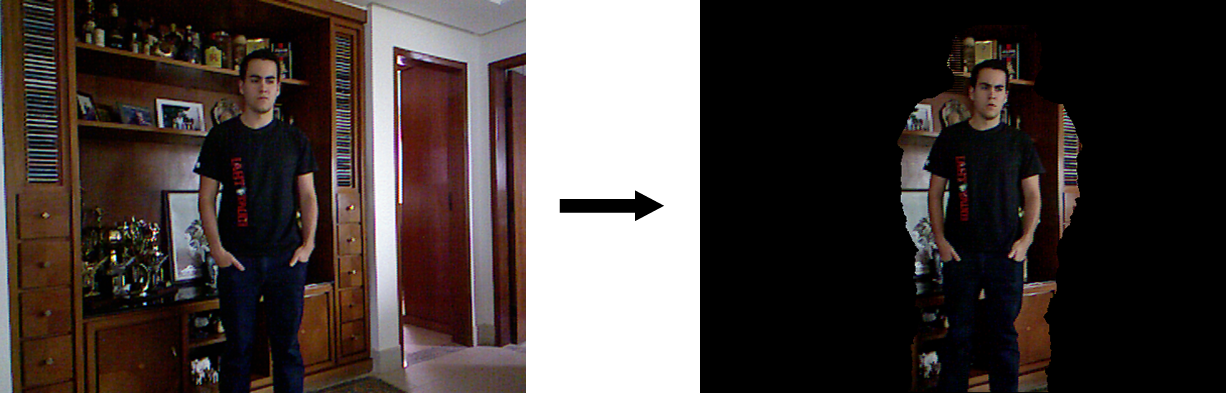
\includegraphics[scale=0.3]{figuras/4.ProblemaEProposta/users-img.png}
			\end{center}
			\caption{Exemplo de uma imagem composta somente pela região em que o usuário se encontra.}
			\label{fig:users-img}
		\end{figure}

		\begin{enumerate}
			\item Obtenção da imagem de entrada composta somente pelo usuário cujo reconhecimento foi requisitado.
			\item Pré-processamento da imagem, ou seja, conversão da imagem em escala de cinza.
			\item Detecção facial na imagem. Caso nenhuma face seja encontrada, retorna ``vazio''. Observa-se que no máximo uma face pode ser encontrada nesta imagem.
			\item Processamento da imagem: uma nova imagem é criada recortando a região da face encontrada. A imagem é, então, redimensionada e equalizada criando assim um padrão de tamanho, brilho e contraste aumentando a acurácia do reconhecimento.
			\item Reconhecimento facial com a técnica \textit{Eigenfaces}.
			\item Retorno do nome do usuário com a face ``mais parecida'' e a confiança do reconhecimento.
		\end{enumerate}

		\begin{figure}[htb]
			\begin{center}
				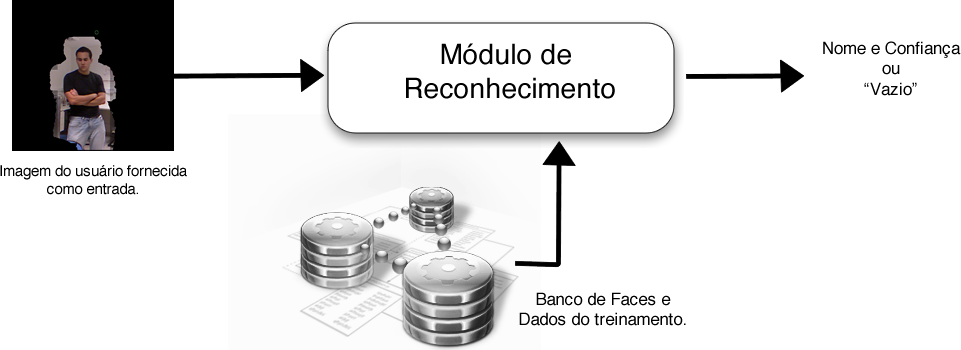
\includegraphics[scale=2.0]{figuras/4.ProblemaEProposta/reconhecimento-simples.png}
			\end{center}
			\caption{Módulo de Reconhecimento do Sistema TRUE.}
			\label{fig:processo-reconhecimento}
		\end{figure}

	% O Módulo de Reconhecimento é dependente do de Rastreamento. Ele ficará ocioso
	% até que chegue uma requisição de reconhecimento de um determinado usuário. A
	% Seção~\ref{sec:rastreamento-reconhecimento} explica mais detalhadamente a
	% relação entre os dois módulos.

	A seguir serão relatados as etapas de Pré-processamento e Processamento da imagem. Depois, serão apresentados em detalhes as etapas de Detecção e Reconhecimento facial.

	\subsection{Pré-processamento e Processamento da Imagem}
		
		As etapas de pré-processamento e processamento das imagens (etapas 2 e 4 mencionadas acima) permitem criar um padrão nas mesmas aumentando a acurácia do reconhecimento. No Sistema TRUE estas etapas consistem em converter a imagem em escala de cinza, recortá-la, redimensioná-la e equalizá-la, criando, assim, padrões de cor, tamanho, brilho e contraste.

		A Figura~\ref{fig:greyscale} exemplifica uma imagem capturada de uma face, a mesma convertida em escala de cinza e depois equalizada. O
		Apêndice~\ref{apend:processamento} contém trechos de código em linguagem C que implementam tais etapas.

		\begin{figure}[htb]
			\begin{center}
				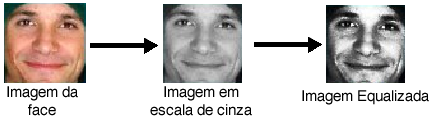
\includegraphics[scale=0.7]{figuras/4.ProblemaEProposta/greyscale.png}
			\end{center}
			\caption{Exemplo de uma imagem de face capturada, a mesma em escala de cinza e depois equalizada. Adaptada de~\cite{shervin}.}
			\label{fig:greyscale}
		\end{figure}

	\subsection{Detecção Facial}

		A detecção facial (etapa 3 mencionada acima) foi desenvolvida utilizando o método \textit{Viola-Jones} apresentado na Seção~\ref{ref:viola-jones}. Este método é adequado para construir uma abordagem de detecção facial rápida e eficaz~\cite{violajones} em tempo real. Além disso, o \textit{Viola-Jones} é implementado pela biblioteca \textit{OpenCV}~\cite{opencv_library} (\textit{Open Source Computer Vision}). Basicamente, o processo de detecção facial procura por uma face em uma imagem pré-processada. Para realizar detecção facial utilizando o método \textit{Viola-Jones} é necessário a utilização de um classificador em cascata, como mencionado na Seção~\ref{subsec:reconhecimento}. Portanto, entre os diversos classificadores em cascata presentes na biblioteca \textit{OpenCV}, o Sistema TRUE utiliza o classificador \textit{haarcascade\underline{ }frontalface\underline{ }alt.xml}, um classificador treinado para detectar faces frontais em imagens.

		% A Figura~\ref{fig:diagrama-deteccao} mostra o fluxo básico do processo de detecção de faces no Sistema TRUE.
		% 	\begin{figure}[H]
		% 	\begin{center}
		% 		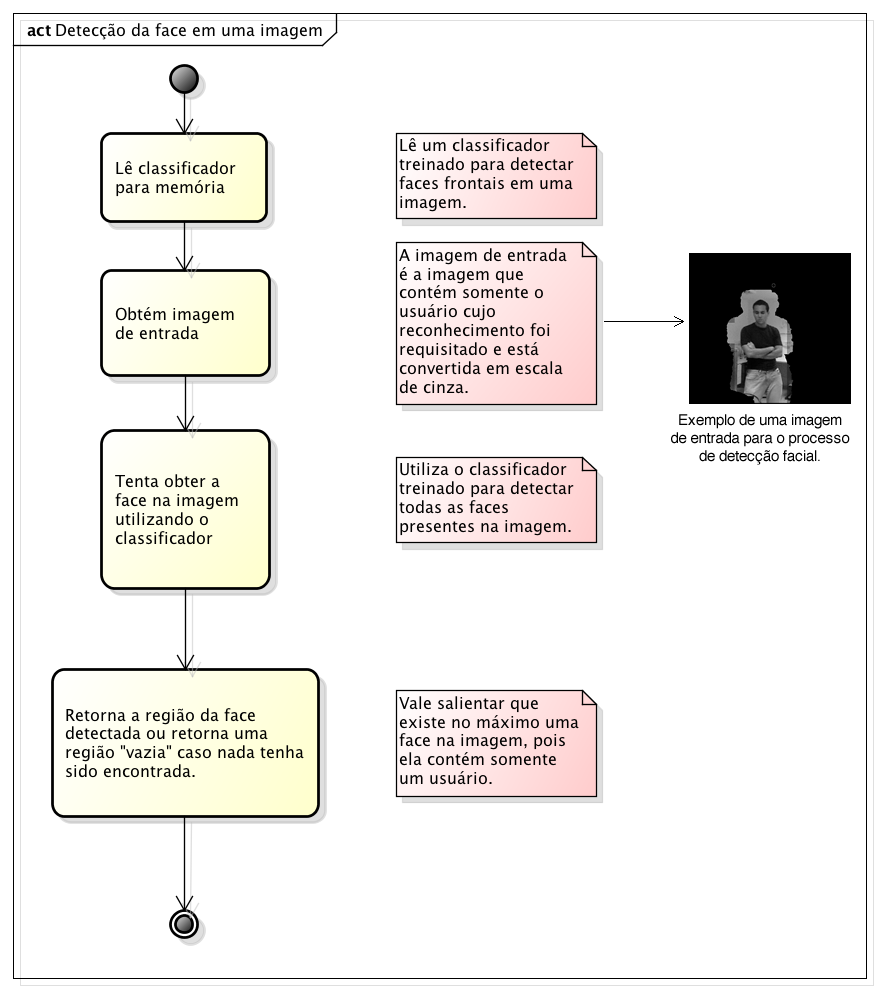
\includegraphics[scale=0.5]{figuras/4.ProblemaEProposta/diagrama-detectar-face.png}
		% 	\end{center}
		% 	\caption{Fluxo de execução do processo de detecção facial no Sistema TRUE.}
		% 	\label{fig:diagrama-deteccao}
		% \end{figure}

		O processo de básico de detecção de faces no Sistema TRUE possui as seguintes etapas:

		\begin{enumerate}
			\item Leitura de um classificador treinado para detectar faces em uma image.
			\item Obtenção da imagem de entrada (esta imagem é composta somente pelo usuário e esta na escala de cinza).
			\item Detecção da face na imagem utilizando o classificador.
			\item Retorno da região da face detectada ou retorno ``vazio'' caso nenhuma face tenha sido encontrada. Observa-se que existe no máximo uma face na imagem, pois contém somente um usuário.
		\end{enumerate}

	\subsection{Reconhecimento Facial com \textit{Eigenfaces}}

		A etapa do reconhecimento facial propriamente dito, correspondente a etapa 5 mencionada acima, foi desenvolvida utilizando a técnica \textit{Eigenfaces} (Seção~\ref{sec:reconhecimento}). Esta técnica consiste em uma técnica bastante satisfatória quando utilizada sobre uma base de faces relativamente grande, permitindo ao sistema inferir, das imagens das faces suas principais características e, partindo delas, realizar o reconhecimento facial utilizando um número reduzido de cálculos~\cite{artigo-eigenface}, permitindo, assim, um reconhecimento em tempo real.

		A base de dados utilizada no Sistema TRUE é formada por imagens no formato PGM (\textit{Portable Gray Map}) com tamanho de 92x112 pixels e em escala de cinza. A base é composta por um banco de faces de alunos voluntários de Ciência da Computação da Universidade de Brasília e por um banco de imagens de faces da Universidade de Cambridge~\cite{cambridgeFaceDb}, mostrado na Figura~\ref{fig:cambridgeFaceDb}. Este último, é formado por imagens de faces de 40 pessoas diferentes. Para cada pessoa, existem 10 diferentes imagens obtidas em diferentes momentos, com diferentes condições de iluminação, diferentes expressões faciais (olhos abertos e fechados, sorrindo e não sorrindo, entre outros) e diferentes detalhes faciais (com e sem óculos). 

		\begin{figure}[H]
			\begin{center}
				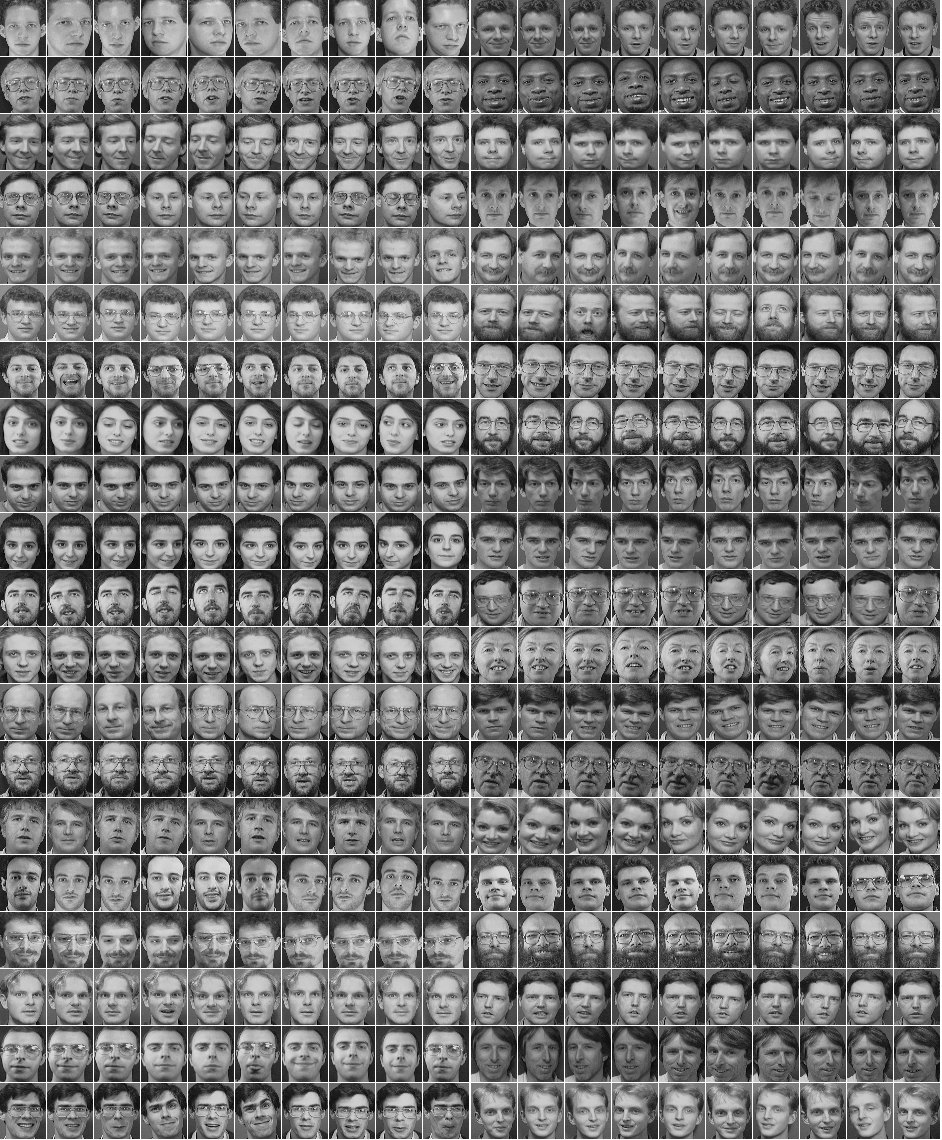
\includegraphics[scale=0.3]{figuras/4.ProblemaEProposta/cambrigdefacedb.png}
			\end{center}
			\caption{Banco de imagens de faces da Universidade de Cambridge~\cite{cambridgeFaceDb}.}
			\label{fig:cambridgeFaceDb}
		\end{figure}

		A Figura~\ref{fig:diagrama-reconhecimento} mostra o fluxo básico do processo de reconhecimento facial no Sistema TRUE.

			\begin{figure}[htb]
			\begin{center}
				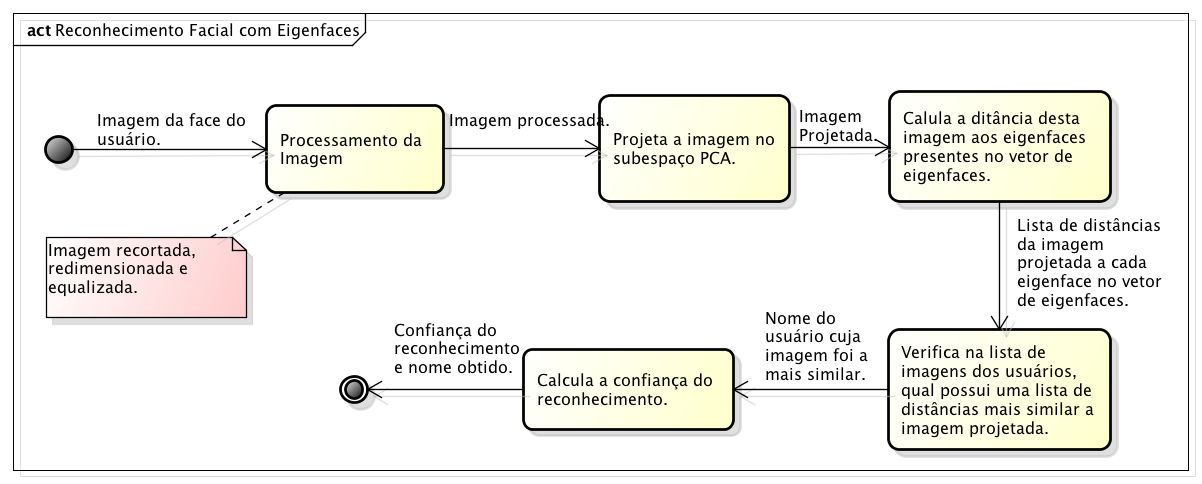
\includegraphics[scale=0.5]{figuras/4.ProblemaEProposta/diagrama-reconhecimento2.png}
			\end{center}
			\caption{Fluxo de execução do processo de reconhecimento facial no Sistema TRUE.}
			\label{fig:diagrama-reconhecimento}
		\end{figure}

		% A primeira etapa consiste na leitura dos dados de treinamento. Esses dados são compostos pela lista dos nomes e imagens das faces dos usuários cadastrados no sistema, pelo vetor de \textit{Eigenfaces}, pela \textit{Eigenface} média e pelos \textit{eigenvalues}.

		% Uma das etapas intermediárias consiste no cálculo da distância entre a imagem projetada no subespaço PCA aos eigenfaces. Inicialmente, o cálculo desta distância era feito utilizando distância euclidiana, porém não apresentava bons resultados em algumas condições. Portanto, este cálculo passou a ser feito utilizando distância Mahalanobis. Contudo, ela também não apresentou bons resultados em alguns casos. Então, alguns testes foram feitos utilizando as duas distâncias de maneira conjunta: uma imagem só é tida como reconhecida quando o resultado das duas distâncias apontarem para a mesma identidade. Com isso, houve uma melhora significativa dos resultados.

		Uma das etapas intermediárias consiste no cálculo da distância entre a imagem projetada no subespaço PCA aos \textit{eigenfaces}. Inicialmente, o cálculo desta distância era feito utilizando distância Euclidiana. Contudo, testes foram realizados com alguns usuários, em que o sistema realizava 20 tentativas de reconhecimento de usuários, e os resultados não foram satisfatórios. Portanto, os mesmos testes foram realizados utilizando distância Mahalanobis. Porém, os resultados também não foram satisfatórios. Então, os mesmos testes foram feitos utilizando as duas distâncias de maneira conjunta: uma imagem só é tida como reconhecida quando o resultado das duas distâncias apontarem para a mesma identidade. Com isso, houve uma melhora significativa dos resultados. Os resultados destes testes são mostrados na Tabela~\ref{tab:distancias}, onde fica claro a melhora dos resultados quando se utiliza ambas distâncias. Nessa tabela, os nome Pessoa1, Pessoa2, Pessoa3, são nomes dados as pessoas cujas fotos estão presentes no banco de imagens de faces da Universidade de Cambrige~\cite{cambridgeFaceDb}.

		\begin{table}[H]
		\begin{center}
			\caption{Resultados do teste de reconhecimento feito com o usuário Danilo utilizando as diferentes distâncias.}
			\label{tab:distancias}
			\begin{tabular}{|c|c|c|c|c|c|c|c|}
				\hline & \bf \begin{sideways}Danilo\end{sideways} & \bf \begin{sideways}Pedro\end{sideways} & \bf \begin{sideways}Ana\end{sideways} & \bf \begin{sideways}Pessoa1\end{sideways} & \bf \begin{sideways}Pessoa2\end{sideways} & \bf \begin{sideways}Pessoa3\end{sideways} & \bf \begin{sideways}Desconhecido\end{sideways}\\
				\hline \bf Euclidiana & 45\% & 40\% & & 5\% & 5\% & 5\% &\\
				\hline \bf Mahalanobis & 40\% & & 15\% & 35\% & 10\% & &\\
				\hline \bf Ambas Distâncias & 75\% & & & & & & 25\%\\
				\hline
			\end{tabular}
		\end{center}
	\end{table}

		A última etapa consiste no cálculo da confiança do reconhecimento. Este cálculo foi feito utilizando a distância da imagem de entrada do usuário à imagem mais similar das imagens de treinamento. O valor da confiança varia de 0.0 a 1.0, em que uma confiança de 1.0 significaria uma ``correspondência perfeita''. A fórmula utilizada para calcular a confiança é uma métrica muito básica que não necessessariamente é muito real, dada pela Fórmula~\ref{eq:confianca}~\cite{shervin}. Nesta fórmula $\displaystyle d_e$ é a distância da imagem de entrada do usuário a imagem mais similar das imagens de treinamento, $\displaystyle n_t$ é o número de imagens utilizadas no treinamento e $\displaystyle n_e$ é o número de \textit{eigenfaces}.


		\begin{equation}
			\label{eq:confianca}
			Confianca = 1 - \frac{\sqrt{\frac{d_e}{n_t * n_e}}}{255}
		\end{equation}






















\section{Módulo de Rastreamento}

	O Módulo de Rastreamento será responsável por rastrear os usuários no ambiente inteligente, determinar a sua localização física em relação ao \textit{Kinect} e gerenciar suas identidades. Para realizar o rastreamento e localização dos usuários é utilizado a biblioteca \textit{OpenNI} (\textit{Open Natural Interaction}). Trata-se de um \textit{framework} que define \textit{APIs} para o desenvolvimento de aplicações de interação natural. Utilizando as imagens de profundidade, a detecção e o rastreamento são feito utilizando subtração de fundo, descrito na Seção~\ref{sec:deteccao-objeto}, e os objetos detectados são representados por suas silhuetas, descrita na Seção~\ref{sec:representacao-objeto}.

	As imagens utilizadas para o rastreamento são imagens de profundidade, exemplificada na Figura~\ref{fig:depthmaps}, providas pelo \textit{Kinect} que são obtidas utilizando o método de Luz Estruturada descrito na Seção~\ref{sec:luz-estruturada}. Tais imagens de profundidade nada mais são que \textit{depth maps} (mapas de profundidade), em que cada pixel da imagem contém o valor estimado da distância em relação ao sensor. O \textit{Kinect} fornece esses dados a uma taxa de $\displaystyle 30 fps$ (\textit{frames} por segundo) com uma resolução $\displaystyle 640px$ x $\displaystyle 480px$.
	

	\begin{figure}[H]
		\begin{center}
			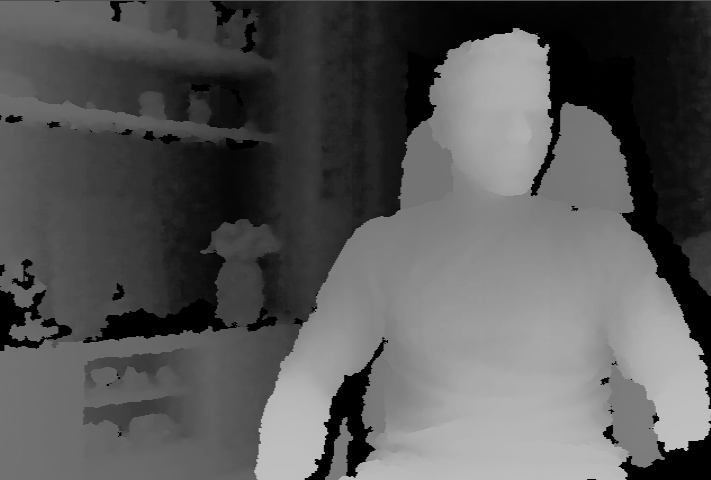
\includegraphics[scale=0.45]{figuras/4.ProblemaEProposta/mapa-profundidade.png}
		\end{center}
		\caption{Exemplo de uma imagem de profundidade fornecida pelo \textit{Kinect}.}
		\label{fig:depthmaps}
	\end{figure}

	Utilizando os mapas de profundidade é possivel calcular as coodernadas $\displaystle (x,y,z)$, em relação ao sensor, de qualquer pixel da imagem. Dessa forma, a posição de um usuário rastreado é determinada utilizando as coordenadas presentes no pixel que representa seu centro geométrico. Sendo assim ao fixar a posição do \textit{Kinect} no ambiente, conseguiremos estimar a localização de qualquer usuário rastreado em tempo real. A Figura~\ref{fig:localizacao} mostra um usuário rastreado pelo Sistema TRUE onde suas coordenadas em relação ao \textit{Kinect} foram estimadas utilizando os valores de profundidade referente ao pixel que representa seu centro de massa geométrico. Os valores das coordenadas $\displaystle (x,y,z)$ estão milimetros.

	\begin{figure}[H]
		\begin{center}
			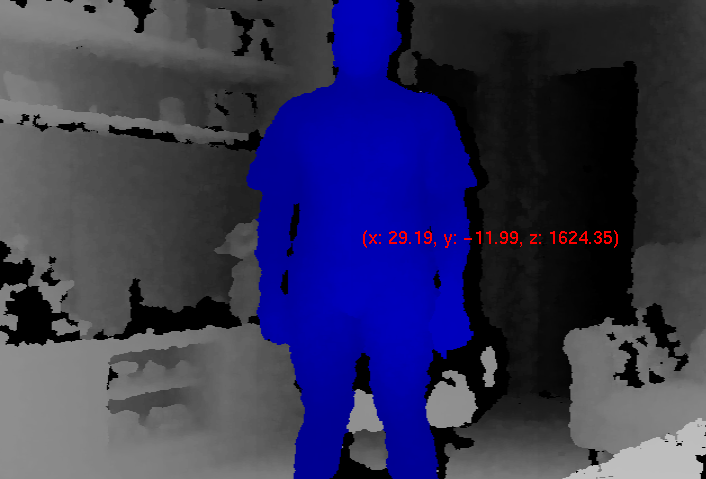
\includegraphics[scale=0.45]{figuras/4.ProblemaEProposta/localizacao.png}
		\end{center}
		\caption{Imagem do Sistema TRUE de um usuário rastreado e localizado.}
		\label{fig:localizacao}
	\end{figure}
	
	
	\begin{figure}[H]
		\begin{center}
			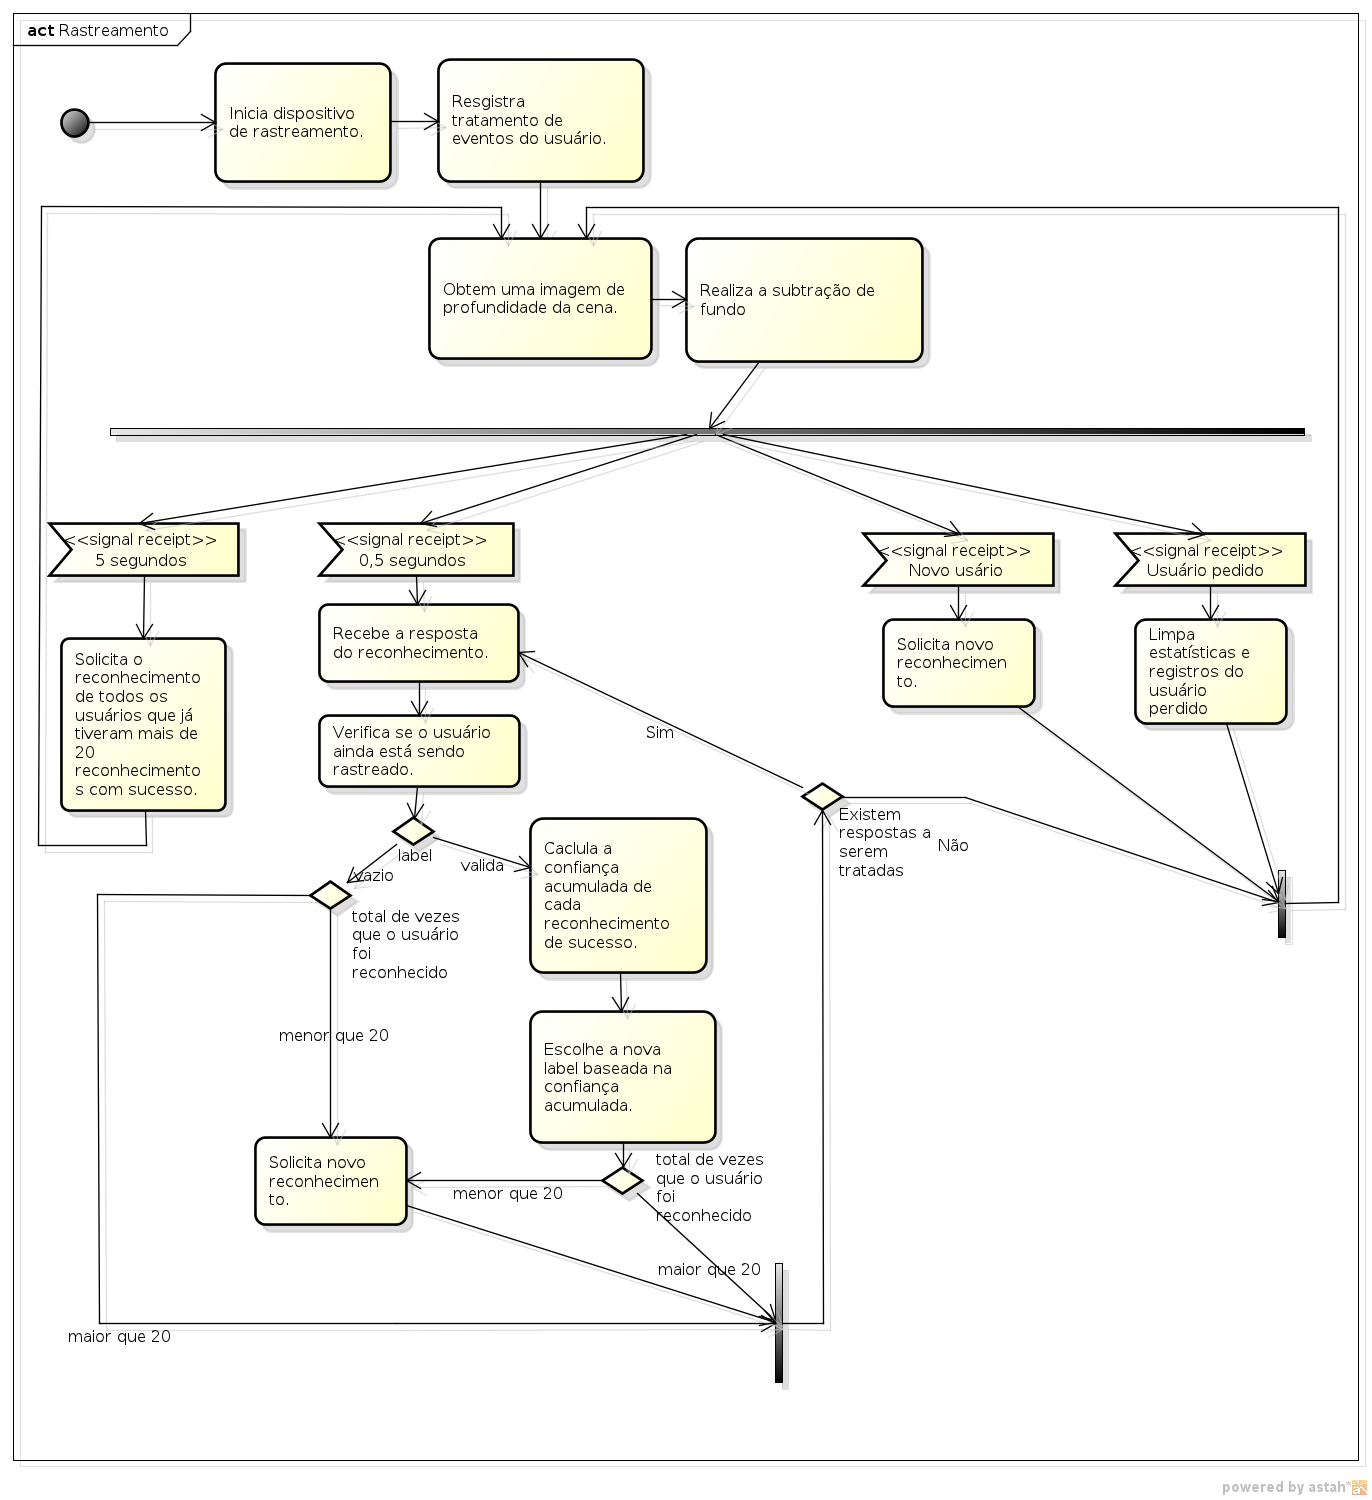
\includegraphics[scale=0.45]{figuras/4.ProblemaEProposta/Rastreamento.png}
		\end{center}
		\caption{Representação das etapas propostas para o rastreamento.}
		\label{fig:processo-rastreamento}
	\end{figure}

\section{Relação Rastreamento e Reconhecimento}
\label{sec:rastreamento-reconhecimento}

	Até agora, foi mostrado como os Módulos de Rastreamento e de Reconhecimento funcionam de maneira isolada, mas não como se relacionam. O Módulo de Rastreamento detém as informações sobre todos os usuários rastreados no ambiente e é responsável por requisitar reconhecimento ao Módulo de Reconhecimento, que deverá acontecer quando um novo usuário for detectado ou quando for necessário reconhecer um usuário já rastreado.

	Basicamente, quando um novo usuário for detectado, a relação entre rastreamento e reconhecimento acontecerá de acordo com as etapas descritas na Figura~\ref{fig:rastreamento-reconhecimento}.

		\begin{figure}[htb]
			\begin{center}
				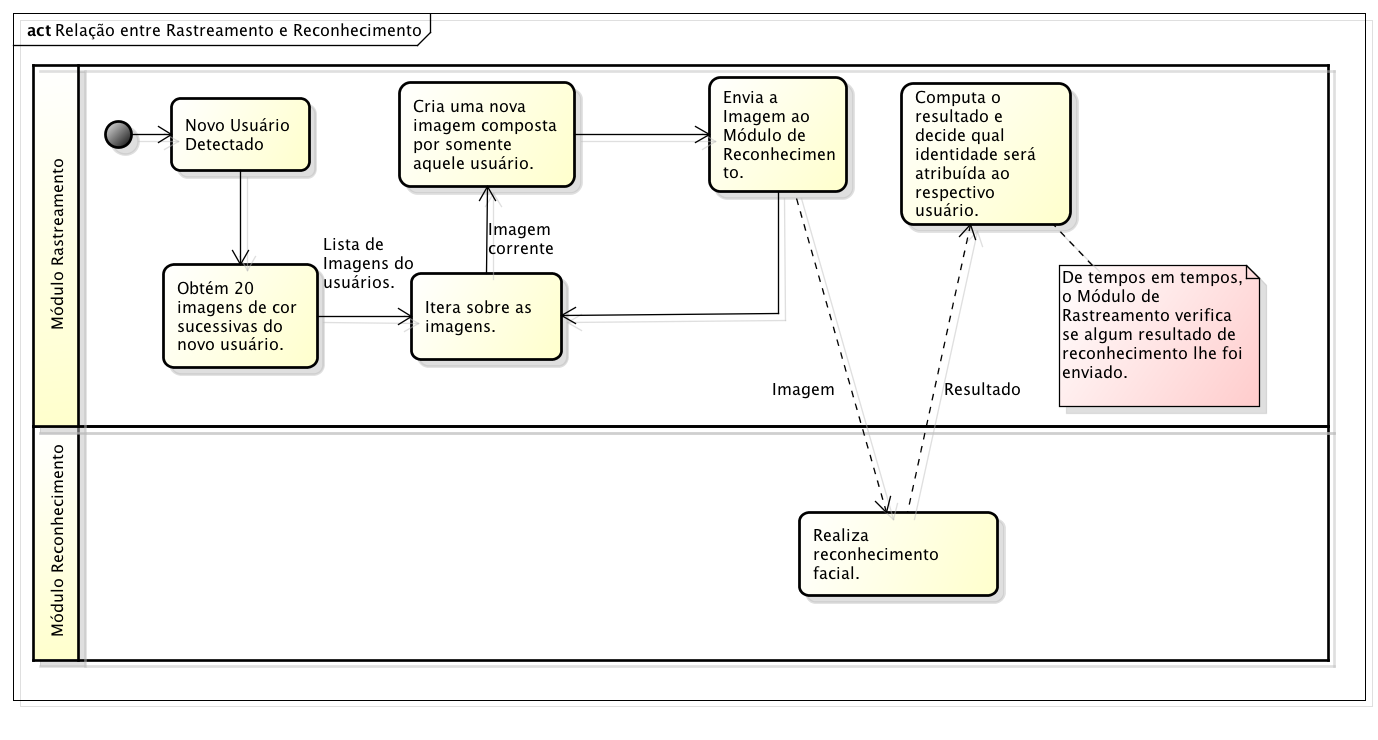
\includegraphics[scale=0.5]{figuras/4.ProblemaEProposta/diagrama-relacao.png}
			\end{center}
			\caption{Representação da relação que o Módulo de Rastreamento terá com o Módulo de Reconhecimento quando um novo usuário for detectado.}
			\label{fig:rastreamento-reconhecimento}
		\end{figure}
	
		% \begin{enumerate}
		%  	\item O Módulo de Rastreamento detecta novo usuário, e obtém um número pré-definido de imagens sucessivas do novo usuário. Para cada imagem, ele cria uma nova imagem de cor contendo somente aquele usuário, como mostrado na Figura (\textbf{colocar a figura aqui}), e a envia para o Módulo de Reconhecimento.
		%  	\item Para cada imagem recebida, o Módulo de Reconhecimento tenta reconhecer o novo usuário e retorna ``vazio'' ou o nome e a confiança do reconhecimento.
		%  	\item O Módulo de Rastreamento verifica se a confiança é maior que um limiar pré-definido, se for ele incrementa o contador que armazena o número de vezes que o usuário foi reconhecido, armazena o nome obtido juntamente com a confiança e calcula qual nome  será atribuído ao novo usuário. Esse cálculo será feito por meio de uma média ponderada utilizando os diferentes resultados obtidos por cada reconhecimento e suas respectivas confianças.
	 % 	\end{enumerate} 
	
	Ao invés de tentar realizar o reconhecimento somente quando novos usuários são detectados, o Sistema TRUE continua a tentar reconhecer os usuários já reconhecidos para melhorar a confiança no reconhecimento. Essas tentativas de reconhecer novamente os usuários ocorrerão em intervalos de tempo pré-definidos seguindo as mesmas etapas de quando um novo usuário for detectado. A única etapa que se difere é a primeira: ao invés de obter várias imagens de um mesmo usuário, são obtidas uma imagem de cada usuário rastreado e as mesmas são enviadas ao Módulo de Reconhecimento.

	Como visto na Figura~\ref{fig:rastreamento-reconhecimento}, ao obter um resultado de reconhecimento para determinado usuário, o Módulo de Rastreamendo deve computar qual identidade será atribuída ao mesmo. Para isso, este módulo mantém para cada usuário o número total de vezes que já foi reconhecido, os diferentes nomes obtidos pelo Módulo de Reconhecimento bem como a confiança média para cada nome e o número de vezes que cada nome foi atribuído ao usuário. Com todos esses dados, a identidade do usuário é escolhida por meio de uma média ponderada entre as confianças de cada nome onde os pesos utilizados são compostos pelo número de vezes que o respectivo nome foi atribuído ao usuário. Vejamos o seguinte exemplo para ilustrar esse cálculo:

	\begin{description}
		Seja João um usuário do ambiente inteligente que está sendo rastreado a algum tempo e que já foi reconhecido algumas vezes. No momento, o Módulo de Rastreamento mantém vários dados sobre o João descritos na Tabela~\ref{tab:joao}. Então, para computar qual identidade será atribuída ao usuário, o Módulo de Rastreamento realiza os cálculos~\ref{eq:joao}. Como o resultado da média ponderada se aproxima mais da confiança do nome João, este foi escolhido como sendo sua identidade.
	\end{description}

	\begin{table}[htb]
		\begin{center}
			\caption{Exemplos de dados de reconhecimento mantidos para cada usuário rastreado pelo Módulo de Rastreamento.}
			\label{tab:joao}
			\begin{tabular}{|c|c|c|}
				\hline \bf Nome & Confiança Média & Número de Vezes \\
				\hline \hline \bf João & 0.947302 & 15 \\
				\hline \bf  Danilo & 0.934010 & 1 \\
				\hline \bf Tales & 0.950320 & 3 \\
				\hline
				\hline \multicolumn{2}{|c|}{\bf Total}  & 19 \\
				\hline
			\end{tabular}
		\end{center}
	\end{table}

	\begin{align}
		\label{eq:joao}
		M_p = \frac{15 * 0.947302 + 1 * 0.934010 + 3 * 0.950320}{19} = 0.947079
	\end{align}

	\begin{align}
	\nonumber & Joao: 0.947079 - 0.947302 = -0.000223\\
		\nonumber & Danilo: 0.934010 - 0.947302 = -0.013292\\
		\nonumber & Tales: 0.950320 - 0.947302 = 0.003018
	\end{align}

	Com todos esses dados de reconhecimento, além dos dados de rastreamento e localização de cada usuário, o Módulo de Rastreamento consegue centralizar todas as informações necessárias de cada usuário. A Figura~\ref{fig:truetotal} exemplifica um usuário rastreado pelo Sistema TRUE onde as informações de localização e identificaçao estão presentes.

	\begin{figure}[htb]
			\begin{center}
				\includegraphics[scale=0.5]{figuras/4.ProblemaEProposta/usuario-identificado.png}
			\end{center}
			\caption{Exemplo de um usuário rastreado e identificado pelo Sistema TRUE.}
			\label{fig:truetotal}
		\end{figure}


\section{Módulo de Registro}

	O Módulo de Registro será responsável por cadastrar novos usuários no sistema e treiná-lo para também reconhecer esse novo usuário. Basicamente, o processo de registro seguirá as seguintes etapas e ilustrada na Figura~\ref{fig:registro}:

		\begin{figure}[hbt]
			\begin{center}
				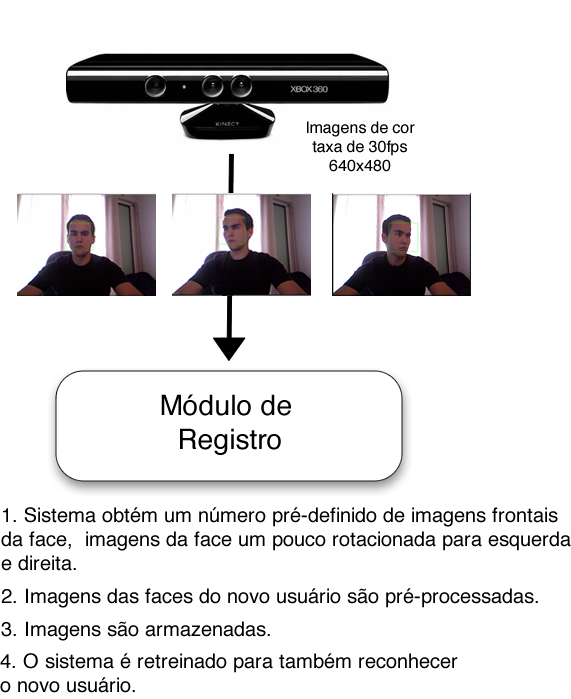
\includegraphics[scale=2.5]{figuras/4.ProblemaEProposta/registro.png}
			\end{center}
			\caption{Etapas de cadastro de um novo usuário no sistema.}
			\label{fig:registro}
		\end{figure}		

		\begin{enumerate}
			\item O novo usuário fica em uma posição fixa e frontal em relação ao \textit{Kinect}. 
			\item O sistema obtém um número pré-definido de imagens frontais do usuário.
			\item O usuário, então, deve rotacionar um pouco a face para a esquerda e o sistema obtém um número pré-definido de imagens do usuário. Depois, deve rotacionar um pouco para direita e o sistema obtém mais imagens do usuário.
			\item As imagens obtidas são processadas: as imagens são convertidas em escala de cinza, novas imagens são criadas recortando a região da face encontrada, as imagens, então, são redimensionadas e equalizadas criando assim uma padrão de tamanho, brilho e contraste nas imagens.
			\item Armazena-se as imagens.
			\item O sistema é treinado para, também, reconhecer esse usuário.
		\end{enumerate}

	Após o treinamento, o sistema \textit{True} reiniciará para que o reconhecimento seja feito utilizando as novas informações obtidas com o treinamento.

\section{Módulo de Integração}
\label{sec:modulo-integracao}

	O Módulo de Integração é responsável pela integração do Sistema TRUE  com o
	Middleware \textit{uOS}. Através desta integração, os dados providos pelo Sistema TRUE (localização
	e identificação dos usuários em um ambiente) são disponibilizadas ao ambiente gerenciado pelo middleware \textit{uOS}
	por meio de serviços. Para integrá-los foi desenvolvido um \textit{driver} para o Middleware se comunicar
	com o Sistema TRUE. Este \textit{driver} foi nomeado de \textit{UserDriver} cujo diagrama de classe
	é mostrado na Figura~\ref{fig:userdriver}. A integração foi feita utilizando
	suporte JNI (\textit{Java Native Interface} - Apêndice~\ref{apend:jni}) uma vez que o Middleware foi desenvolvido em JAVA e o Sistema TRUE em C++.

	% O Módulo de Integração é responsável pela integração do Sistema TRUE  com o
	% Middleware \textit{uOS}. Os dados providos pelo Sistema TRUE (localização
	% e identificação dos usuários em um ambiente) são informações de
	% contexto relevantes para ambientes inteligentes. O Middleware \textit{uOS} foi
	% escolhido como meio de fornecê-las as diversas aplicações no ambiente. Então,
	% para integrá-los foi desenvolvido um \textit{driver} para o Middleware se comunicar
	% com o Sistema TRUE. Este \textit{driver} foi nomeado de \textit{UserDriver} cujo diagrama de classe
	% é mostrado na Figura~\ref{fig:userdriver}. A integração foi feita utilizando
	% suporte JNI (\textit{Java Native Interface} - Apêndice~\ref{apend:jni}) uma vez que o Middleware foi desenvolvido em JAVA e o Sistema TRUE em C++.

	\begin{figure}[htb]
		\begin{center}
			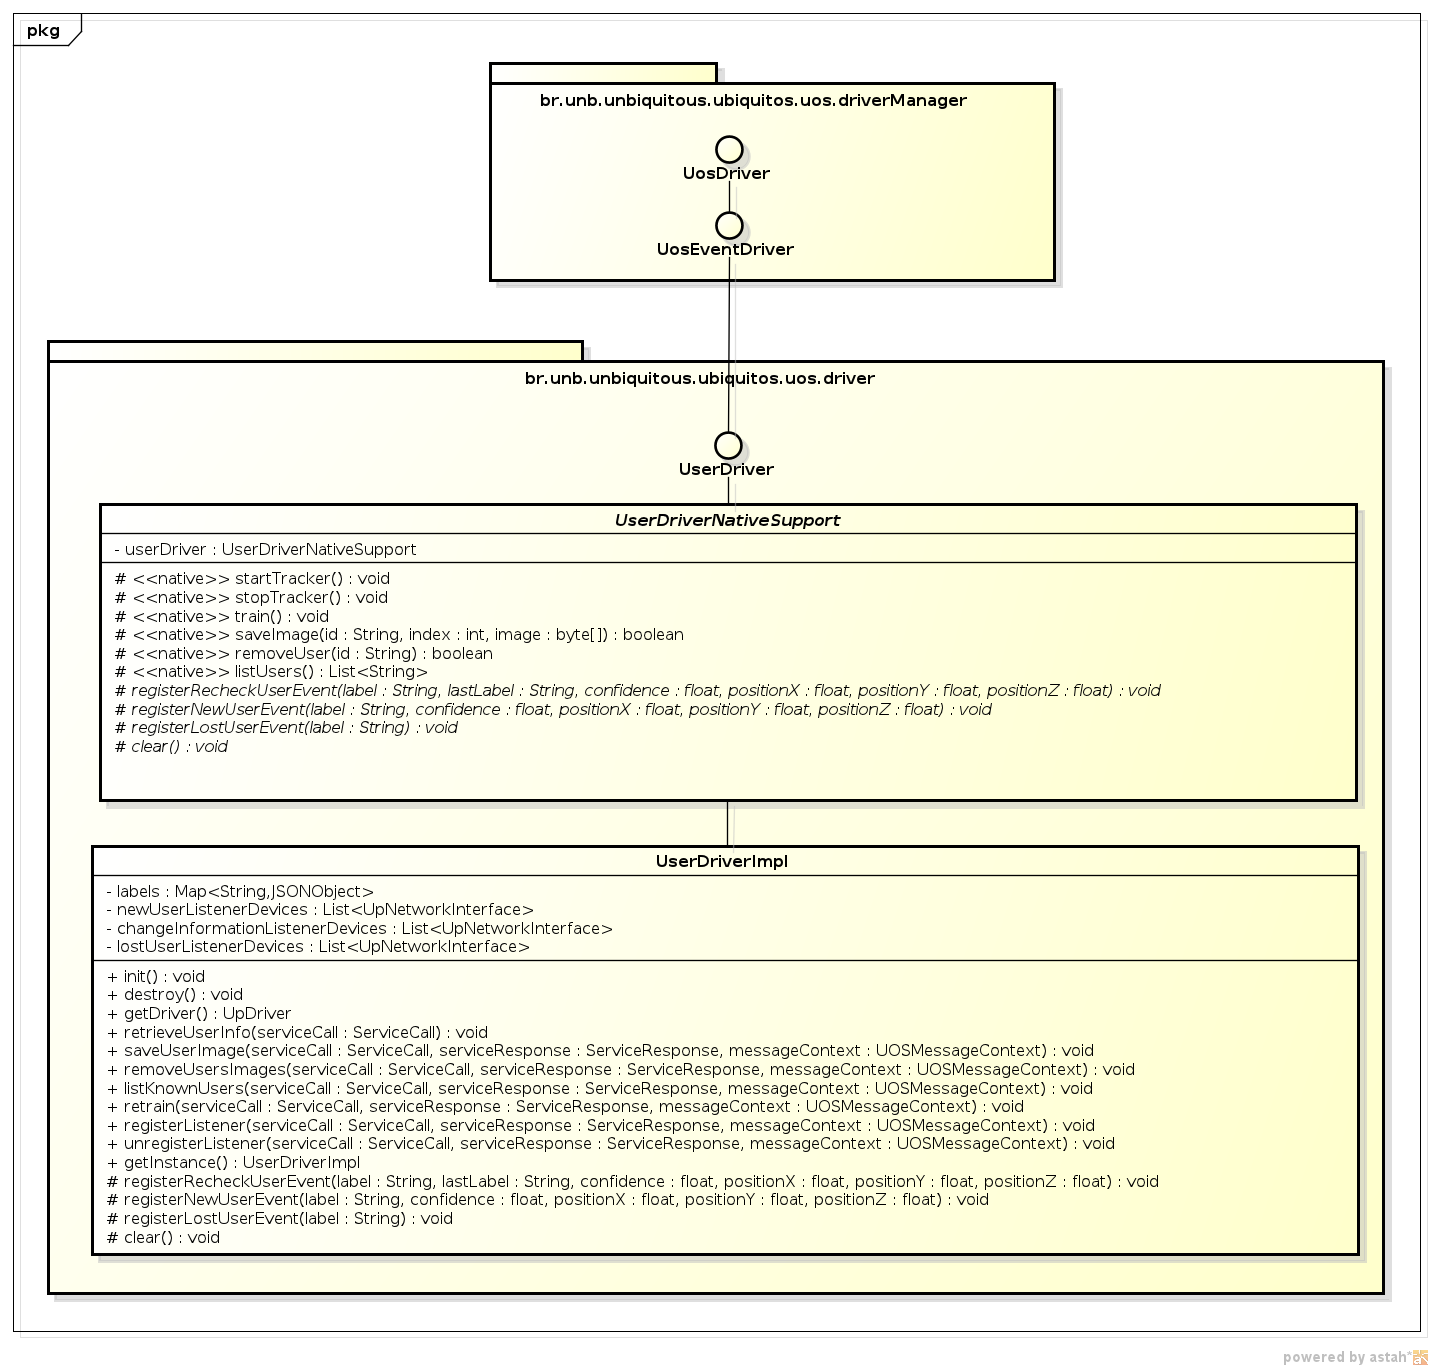
\includegraphics[scale=0.45]{figuras/4.ProblemaEProposta/diagrama-classe-userdriver.png}
		\end{center}
		\caption{Diagrama de Classe do UserDriver.}
		\label{fig:userdriver}
	\end{figure}

Os métodos do \textit{UserDriver} podem ser divididos basicamente em três grupos, isto é, métodos de inicialização, métodos nativos e de serviços e eventos:

\begin{itemize}
	\item \textbf{Métodos de Inicialização}: métodos responsáveis pela inicialização do Sistema TRUE e pelo registro dos serviços que o \textit{driver} possui e os eventos que pode gerar.

	\item \textbf{Métodos Nativos}: métodos declarados no \textit{driver} que permitem acessar alguns métodos implementados pelo Sistema TRUE. Tais métodos permitem que o \textit{UserDriver} tenha controle sobre o sistema, podendo iniciá-lo, encerrá-lo, retreiná-lo e, até mesmo, cadastrar e remover novos usuários a qualquer momento. Para implementar os métodos nativos foi utilizado JNI (\textit{Java Native Interface}), descrito no Apêndice~\ref{apend:jni}.

	\item \textbf{Serviços e Eventos}: são os métodos que implementam os serviços que o \textit{UserDriver} disponibiliza às aplicações presentes no ambiente e os eventos que pode gerar. 

	% Nestes serviços incluem consultas as informações (nome e localização) de qualquer usuário presente no ambiente, listagem dos usuários no ambiente, cadastro e remoção de novos usuário do Sistema TRUE e retreino do mesmo, e registro de \textit{listeners} que ``escutam'' os eventos gerados pelo driver. Nos eventos incluem evento de um novo usuário detectado, evento de um usuário perdido, evento de quando a identidade do usuário é corrigida e um outro evento que é gerado de tempo em tempo atualizando a posição de todos os usuários no ambiente.

\end{itemize}



	O \textit{UserDriver} disponibiliza às aplicações registradas no
	\textit{middleware} os seguintes serviços:

	\begin{itemize}
		\item \textbf{Consultas as informações dos usuários no ambiente}: através dessas consultas, as aplicações tem acesso ao nomes, emails, posições correntes e confiança do reconhecimento de todos os usuários presentes no ambiente.
		\item \textbf{Cadastro}: as aplicações podem cadastrar novos usuários fornecendo ao \textit{UserDriver} o nome, o email e as imagens do novo usuário.
		\item \textbf{Treino do sistema}: após cadastrar novos usuários as aplicações podem retreinar o sistema para poder reconhecer o novo usuário cadastrado.
		\item \textbf{Remoção}: as aplicações podem remover usuários cadastrados fornecendo o email do usuário.
		\item \textbf{Registro de \textit{listeners}}: as aplicações podem registrar \textit{listeners} para ``escutar'' os eventos gerados pelo \textit{UserDriver}.
	\end{itemize}

Além dos serviços, o \textit{UserDriver} gera os seguintes eventos:

	\begin{itemize}
		\item \textbf{Novo Usuário}: evento gerado assim que um novo usuário foi detectado pelo Sistema TRUE.
		\item \textbf{Usuário Perdido}: evento gerado assim que um usuário deixou de ser rastreado pelo Sistema TRUE.
		\item \textbf{Atualização dos dados do usuário}: evento gerado a cada cinco segundos atualizando os dados de todos os usuários rastreados.
	\end{itemize}

	O Módulo de Integração se comunica diretamente com os Módulos de Rastreamento e de
	Registro através do \textit{UserDriver}. Enquanto a comunicação com o Módulo de
	Registro acontece somente quando alguma aplicação solicita o cadastramento ou a remoção
	de usuários, a comunicação com o Módulo de Rastreamento acontece constantemente:

	\begin{itemize}
		\item a cada 5 segundos o Módulo de Rastreamento envia informações correntes sobre todos os usuários no ambiente atualizando as informações que o Módulo de Integração detém;
		\item sempre que um usuário entra ou sai do ambiente o Módulo de Rastreamento informa o Módulo de Integração.
	\end{itemize} 

	Através do \textit{UserDriver}, o Middleware \textit{uOS} tem acesso às
	informações sobre identidade e localização dos usuários presentes no ambiente em
	tempo real. Tais informações ficam disponíveis a qualquer aplicação registrada
	no Middleware.

